\documentclass[11pt]{article}
\usepackage[margin=0.8in]{geometry}
\usepackage{amsmath,amssymb,booktabs,graphicx}
\usepackage{enumitem,microtype,float}
\usepackage[hidelinks]{hyperref}
\hypersetup{pdftitle={ODE-FFN: Progress Report 2},pdfauthor={Zhizhe Zhang}}
\setlist{nosep,leftmargin=*}
\setlength{\parskip}{2pt}
\makeatletter
\renewcommand\section{\@startsection{section}{1}{\z@}%
 {6pt\@plus2pt\@minus2pt}{2pt}{\normalfont\large\bfseries}}
\makeatother
\newcommand{\norm}[1]{\lVert#1\rVert}
\title{\vspace{-1.6em}\textbf{ODE-FFN: Progress Report 2}\\[3pt]
\large Independent Study --- Deep Learning}
\author{Zhizhe Zhang\\NYU Shanghai}
\date{1 November 2026\quad(Draft)}
\begin{document}
\maketitle
\vspace{-2.8em}

\section{Project overview}
We study whether an internal dynamical structure can improve the FFN in JiT,
which predicts a clean image from a noisy image and time. Since Report 1,
nonlinear-flow and operator-direction experiments have produced useful synthetic
results, with limited transfer. The current CIFAR-10 experiment has not yet
established an image-generation advantage.

\section{From a linear flow to a nonlinear response}
The original layer uses the degree-$K$ Taylor map $T_K(sP)h\approx\exp(sP)h$.
We instead considered
$dy/dr=Py-y^{\odot3}$, whose cubic part has the exact elementwise solution
\begin{equation}
\phi_s(u)=\frac{u}{\sqrt{1+2su^2}},\qquad
\phi_s'(u)=(1+2su^2)^{-3/2}.
\label{eq:response}
\end{equation}
The tied split beats the old ODE but loses to ordinary controls. Its useful
control is the free ISRU FFN,
\begin{equation}
f(h)=W_2\phi_{0.6}(W_1h),\qquad
W_1=W_2=I+0.3P+0.045P^2\quad\text{at initialization}.
\label{eq:ffn}
\end{equation}
The matrices train independently, without an adaptive duration or tied generator.
This tests the response and initialization together, not an isolated activation.

\section{Synthetic experiment: where does ISRU help?}
\textbf{Purpose.} Test the response against ordinary SwiGLU. Velocity networks
use width 64, three blocks, batch 512, AdamW at $3\!\times\!10^{-4}$, clipping
at 1, and 5,000 updates. Analytical conditional velocities are used for
evaluation; training uses noise--data pairs without oracle supervision.
Product16 is a rotated mixture with independent bimodal latent coordinates.
Dependent signs change their dependence while preserving latent marginals;
the half mixture combines these two laws.

\begin{table}[H]
\centering\small
\begin{tabular}{lrrr}
\toprule
Target & Free ISRU & SwiGLU64 & SwiGLU160\\
\midrule
Gaussian 2D &0.005429&0.004192&0.004557\\
Ring8 &0.016694&0.017904&0.013921\\
Product16 &0.037159&0.164398&0.078178\\
Dependent signs &0.085073&0.051075&0.039790\\
Half mixture &0.163557&0.192344&0.113254\\
\bottomrule
\end{tabular}
\caption{Oracle field MSE at 5k (lower is better). SwiGLU64 nearly matches
ISRU's parameter count; SwiGLU160 is wider. Compare within each target.}
\label{tab:synthetic}
\end{table}
\vspace{-0.6em}
\textbf{Observation.} Product16 field error is 52.5\% below SwiGLU160, using
58.5k versus 95.8k parameters. Its sliced Wasserstein distance is 0.09290 versus
0.09784; SwiGLU64 already reaches 0.09276. The field gain is not an equally
clear generation gain. Ring8 and the half mixture beat SwiGLU64 but lose to
SwiGLU160. Dependent signs reverse the Product16 ordering. The half mixture
retains every Product16 component location, so component count alone cannot
explain the reversal.

\newpage
\section{CIFAR-10 transfer: fitting and generation remain different}
\textbf{Purpose and setup.} Test ISRU in unconditional pixel JiT against matched
and wider SwiGLU. All share width 192, six blocks, three heads, patch 4,
non-FFN initialization and batches. Parameter counts are 2.870M/2.873M/4.204M.
We use 45k training/5k validation images, batch 512, AdamW at $10^{-4}$,
500-step warmup then constant LR, betas $(0.9,0.95)$, clipping at 1,
and EMA decay 0.9999.

The model predicts $D_\theta(z_t,t)$, with standard Gaussian noise $e$ and $\epsilon$, $z_t=tx+(1-t)e$, and
$t=\operatorname{sigmoid}(0.8\epsilon-0.8)$. Training minimizes
$\mathbb{E}\norm{(D_\theta-x)/\max(1-t,0.05)}^2$, averaged over pixels.
Sampling uses 50 intervals, Heun then final Euler, without class guidance.
Training is ongoing toward 50k updates. This draft includes validation through
40k and all completed FIDs through 25k; the final endpoint is unavailable.

\begin{figure}[H]
\centering
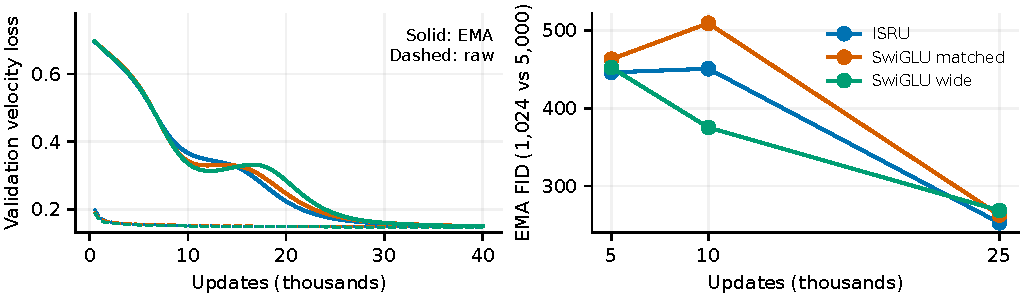
\includegraphics[width=\textwidth]{figures/cifar-dynamics.pdf}
\caption{Left: fixed validation loss, raw weights dashed and EMA solid.
Right: all completed EMA FIDs, using 1,024 generated and 5,000 reference images
at each point. These are interim scores, not 50k-image benchmark FIDs.}
\label{fig:cifar}
\end{figure}
\vspace{-0.6em}
\textbf{Observation.} At 25k, FID is 252.96/262.93/268.74 for ISRU/matched/wide
SwiGLU. These remain poor absolute scores. The order also changes: at 10k,
wide SwiGLU has 375.26 versus ISRU's 450.60. The 25k gap does not establish
architecture superiority.

\begin{figure}[H]
\centering
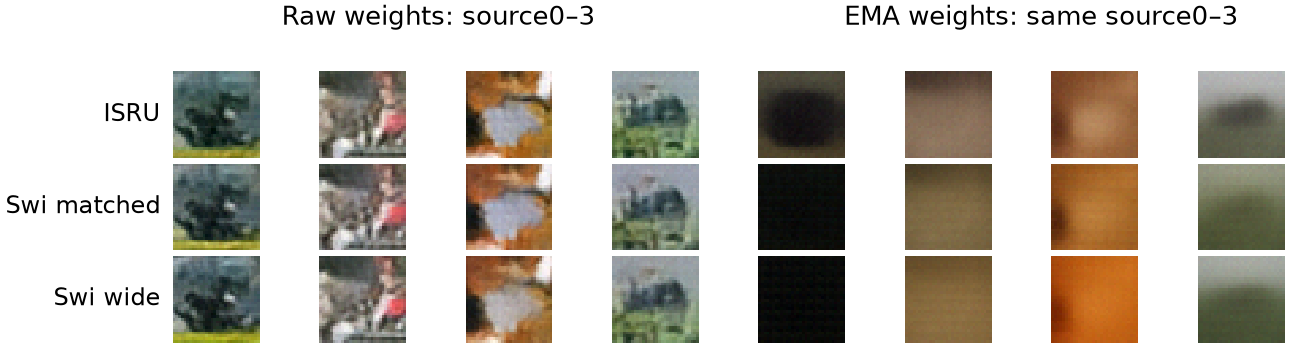
\includegraphics[width=0.96\textwidth]{figures/cifar-cases.png}
\caption{Fixed cases 0--3 at 25k, using identical starting noise across methods
and raw/EMA weights. Raw samples retain more texture; EMA samples remain
dominated by blurred color regions. Cases were selected by index, not quality.}
\label{fig:cases}
\end{figure}
\vspace{-0.6em}
ISRU's raw/EMA validation losses are 0.14834/0.17124 at 25k and
0.14717/0.14905 at 40k. Wide SwiGLU's 40k raw loss is lower, 0.14613.
EMA retains 8.2\% of its initial parameters at 25k, with an approximately
10k-update averaging horizon. This observed lag complicates early FID:
parameter averaging is not output averaging, and cannot alone explain the
generation deficit. Raw-weight FID remains unmeasured.

\newpage
\section{What the learned matrices tell us}
\textbf{Purpose.} Check how the free matrices affect the response's sensitivity.
For Eq.~\eqref{eq:ffn}, the complete bare-FFN Jacobian is
\begin{equation}
J_f=W_2\operatorname{diag}\!\left((1+1.2(W_1h)^2)^{-3/2}\right)W_1,
\qquad \norm{J_f}_2\leq\norm{W_2}_2\norm{W_1}_2.
\label{eq:jac}
\end{equation}
The cubic response alone is nonexpansive; the learned maps need not be.
Normalization, conditioning and residual paths further change the full block
Jacobian. An exact local subflow does not guarantee predictor stability.

\begin{figure}[H]
\centering
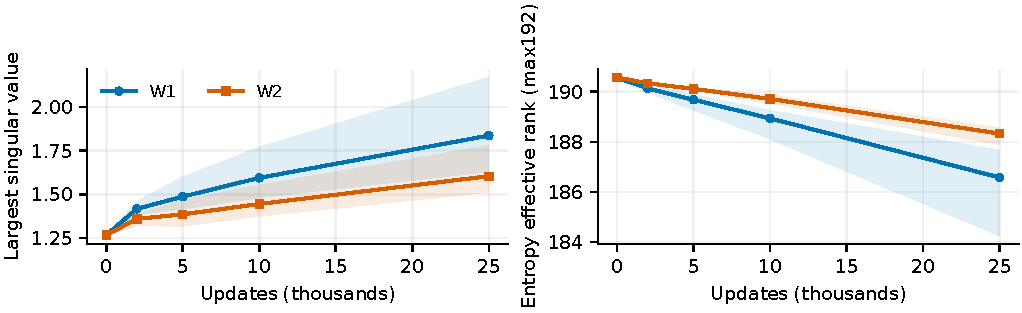
\includegraphics[width=\textwidth]{figures/matrix-trajectories.pdf}
\caption{Raw ISRU matrix histories. Lines average six blocks; shaded bands
show their minimum--maximum range, not uncertainty intervals. Effective rank
is $\exp(-\sum_i p_i\log p_i)$, where $p_i=\sigma_i/\sum_j\sigma_j$.
These free maps are W1/W2, not a uniquely defined trained generator P.}
\label{fig:matrices}
\end{figure}
\vspace{-0.6em}
\textbf{Observation.} Mean largest singular values change from 1.27 at initialization to 1.84 for W1 and 1.60 for W2 at 25k. Mean effective ranks remain 186.6 and 188.3 out of 192.

These finite trajectories show learned anisotropy, rather than singular-value
flattening. They do not identify a matrix instability as the cause of poor FID,
and do not yet justify adding a spectral penalty.

\section{A separate test of input-dependent operator directions}
\textbf{Purpose.} Test input-dependent orthogonal rotations,
$Q(h)T_K(s(h)P)Q(h)^\top h$. On eight 2D modes embedded in 128D,
frame K2 reduces field MSE from 0.002729 to 0.000685 per ambient coordinate.
SwiGLU192 reaches 0.003095. Generated projections recover eight visible clusters.
Yet same-frame K1 reaches 0.000713 and better tangent sliced Wasserstein
distance, 0.1950 versus 0.2041. With full-dimensional variation, K2 tangent
distance is 0.3173 versus SwiGLU192's 0.2471.

At fixed input, this rotation preserves P's eigenvalues and singular values
while changing its action. Thin-data gains therefore support direction
conditioning, not a K2-specific benefit or robust transfer. Spectra alone
cannot characterize the useful nonlinear map.

\section{Hypotheses for the next two weeks}
\begin{enumerate}
\item \textbf{EMA lag accounts for a substantial part of the early image deficit.}
Finish the registered 50k run. Compare raw/EMA checkpoints with identical
noise, counts and sampler; predict a larger quality gap at 25k than 50k.
Retain the registered EMA results and label this additional diagnostic.
\item \textbf{The Product16 advantage persists after longer training.}
Continue ISRU and both SwiGLU controls on Product16 and dependent signs
under one longer budget, retaining curves and sampling metrics. A closing
gap would suggest a finite-budget effect. If it persists, isolate the response
at fixed matrix initialization before attributing it to ODE structure.
\end{enumerate}
\end{document}
